% !TeX root = ../report.tex
% !TeX spellcheck = en-GB
% !TeX encoding = UTF-8
\chapter{Dredging principles and applications}\label{chap:dredgingprocess}
This chapter describes the dredging task in some detail. Readers familiar with dredging and commonly used terminology can skip this chapter, since no new information will be provided. It first describes basic principles, applications and tools applicable by the used machinery for the use-cases.

\section{Basic dredging application}\label{sec:basic dredging applications}
\citet{training_institute_for_dredging_ingewijden_2008} defines dredging as the underwater removal of soil and its transport from one place to another for the purpose of deepening or making profitable use of the removed soil. They make an distinction between nine types of operations: dredging for prosperity, dredging in ports an
d channels, exploitation of agricultural resources, mineral dredging, coastal protection, land reclamation, infrastructural projects, improvement of the environment and trenches for cables and pipelines.

All three described use-cases are of the maintenance type. \citet{van_der_schrieck_dredging_2014} states that the issue in maintain existing waterways and harbours, preserve the depth of the bed by regular removing silt. In canals and ports basins, where currents are low, the sediment is mostly fine-grained silt and sludge. Where currents are stronger, as in access channels in tidal zones, or rivers, the sediment is sand. He further describes that a characteristics of this kind of work is the weak cohesion of the soil to be removed, since it consist of recently deposited sediment and no significant consolidation has taken place yet.

A special kind of maintenance dredging is sanitation dredging which is a process specially designed for contaminated sediment. Just in the way, sediment settles in rivers, harbours and deltas so does heavy metal, inorganic and aromatic compounds. Especially downstream of industrial areas. When these contaminated sediments become a risk towards public health and environment it needs to be removed with care and precision.

\section{Commonly used vessels and equipment}\label{sec:Commonly used vessels and equipment}
Common dredge tools used during maintenance work are listed below, of this list backhoes and suction dredgers are mostly used during port maintenance. \citet{vlasblom_designing_nodate} states that dredgers can be divided in mechanical dredgers and hydraulic dredgers. Where the difference lies in the way the soil is excavated; either mechanical or hydraulic.

\subsection{Mechanical Dredgers}\label{sec:Mechanical Dredgers}
They work by removing soil and sediment from the submerged soil bed by mechanically excavating it and transporting it to a storage location, such as a \gls[first]{gls-hopper}.

The various types of mechanical dredgers won't be described in this section, since the \gls[first]{acr-AOD} used in our uses-cases will be of a hydraulic type.

\subsection{Hydraulic Dredger}
These types of dredgers work by removing and transporting soil from the seabed. They use a hydraulic system, were the necessary work needed for mass transportation is deliver by a pump. The soil is transported as a \gls[first]{gls-slurry} and usually stored in a dedicated place such as a \gls{gls-hopper}.

\subsubsection{Plain Suction Dredger}
\citet{vlasblom_designing_nodate} describes a plain suction dredger as an stationary dredger, consisting of a pontoon anchored by one or more wires an with at least one sand pump, that is connected to a suction pipe. The discharge of the dredged material can take place via a pipeline or via a barge-loading installation. During sand dredging the dredger is moved slowly forwards by a set of winches.

\subsubsection{Trailing suction hopper dredger}
The \gls[first]{acr-TSHD} is a seagoing ship equipped with one or two suction tubes, a pump installation and a \gls{gls-hopper} with multiple bottom doors and one or more overflows. A \gls{gls-draghead} attached to each suction tube and is trailed across the sea bed to loosen the soil before it is pumped up~\cite{van_der_schrieck_dredging_2014}. This soil is stored in a \gls{gls-hopper} which is periodically discharged, at an designated location, through dumping or pumping out.

\subsubsection{Auger Suction Dredger}
According to \citet{vbko_vereniging_van_waterbouwers_in_bagger_kust_en_oeverwerken_voortgezette_1998} an \gls[first]{acr-ASD} consists of a double symmetrical Archimedes screw, also called an auger, surrounded with a steel protective cover and a flexible rubber curtain. This auger is lowered on a rigid arm and positioned on the soil bed, where it cuts the material and actively transports in to the centre, where it is sucked away by a dredge pump. Because the complete dredging process takes place behind a flexible rubber curtain and the auger guides all material towards the suction mouth, this types of dredgers are well suited for sanitation maintenance.

\begin{RoyalFigure}[htb]{AUGER SUCTION DREDGER~\cite{vbko_vereniging_van_waterbouwers_in_bagger_kust_en_oeverwerken_voortgezette_1998} }
  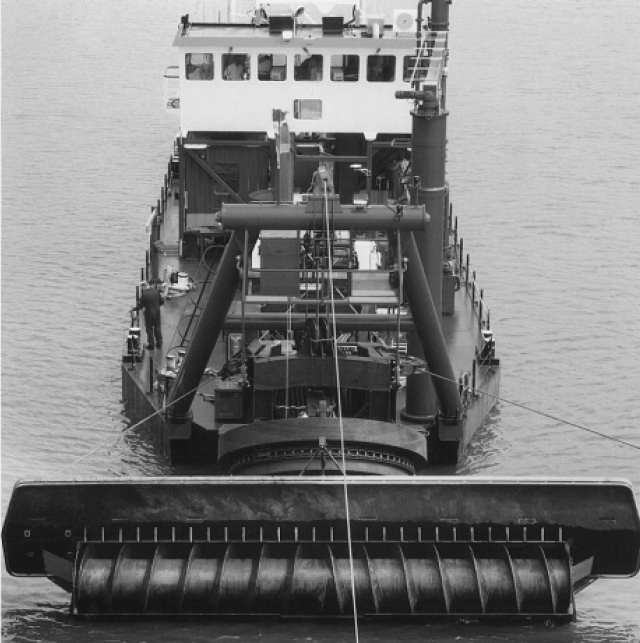
\includegraphics[width=\textwidth]{wormwielzuiger.png}
\end{RoyalFigure}

\subsubsection{Cutter Suction Dredger}
According to \citet{vlasblom_designing_nodate} a \gls[first]{acr-CSD} is a stationary dredger equipped with a cutter device (cutter head)  which excavate the soil before it is sucked up by the flow dredge-pump. During this operation the dredger moves around a spud pole by pulling and slacking on the two fore sideline wires. This type of dredger is accurate and can cut almost all types of sediment.

\section{Hydraulic dredging principals}
According to \citet{van_den_berg_ihc_2013} hydraulics systems are the de-facto industry of transportation for dredged sedimented, or \gls{gls-slurry}; Hydraulic systems consists of pipes, either flexible or rigid, combined with centrifugal pumps, a suction mouth and a discharge unit. These components are usually placed in series. A \gls{gls-slurry} moving through a hydraulic system experiences friction, both from shearing of a fluid along a wall and internal shearing of the fluid itself. This friction results in a pressure drop along these components. Coupled with a pressure drop needed to overcome a height difference, result in a needed pressure, which the pump has to deliver for a certain flow-rate.

The section below shortly describe the workings of two main components in this hydraulic system, namely a dredge-pump and a \gls{gls-draghead}.

\begin{RoyalNote}{OUT-OFF SCOPE}
  Two of the use-cases mention that additional constrains such as a flexible dredge line to shore can be added to the equation. Since the dredge bot does not have a holding space to store collected sediment this is part of the normal operation. It was however opted, to not applied these additional constraints, due to a time constraint on the assignment as a whole.
\end{RoyalNote}

\subsection{Dredge pump}
In order to transport \gls{gls-slurry} with a particular density and velocity through a pipeline, a pressure, equal to the sum of all the resistances and geodetic head must be generated. A pump supplies this pressure~\cite{van_den_berg_ihc_2013}. Assuming a steady flow, the pump basically increases the Bernoulli head of the flow between point 1, the eye and point 2, the exit~\cite{white_fluid_2011}.

\subsection{Auger dredge head}
An auger \gls[first]{gls-umbilical} This method ensures an extremely quit cutting and mixing process with little spillage and turbidity in the surroundings. The large working width of the auger makes it extremely suited to dredge thin possible polluted, layers at a relatively high production rate~\cite{van_der_schrieck_dredging_2014}.

\begin{RoyalFigure}[htb]{SCHEMATIC DRAWING OF AN AUGER DREDGE HEAD~\cite{wetering_ihc_mti_crawler_dredger_final_report_20018} }
  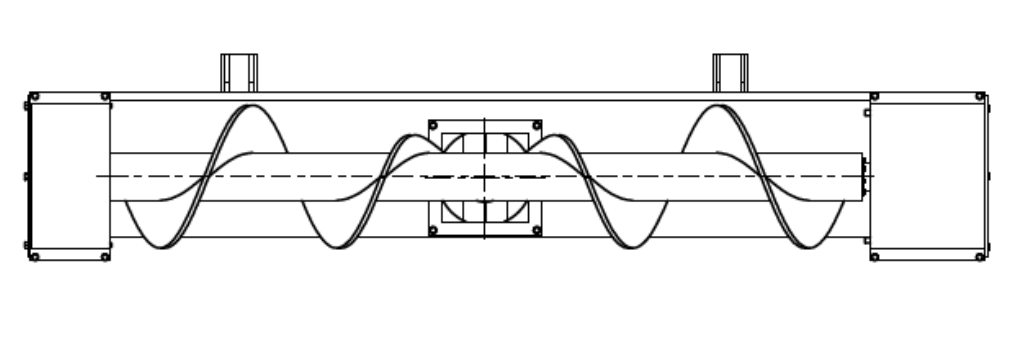
\includegraphics[width=\textwidth]{dredgehead.png}
\end{RoyalFigure}

The auger is in effect a screw conveyor which guiding the material towards the suction head. \citet{perry_2007} states that the screw conveyor one of the oldest and most versatile conveyor types is. It consists of a helicoid flight mounted on a pipe which turns in a trough. Screw conveyors are well standardized, using~\citet{international_standard_iso_neniso_1981} empirical gathered factor values for filling rates and progress resistance.

\begin{RoyalNote}{ASSUMPTION}
	The assumption is made that the hydraulic system, consisting of flexible pipes and pump are the limiting factor in the mass flow, and that the auger simply delivers what is needed.
\end{RoyalNote}
